%
% ---------------------------------------------------------------
% Copyright (C) 2012-2018 Gang Li
% ---------------------------------------------------------------
%
% This work is the default powerdot-tuliplab style test file and may be
% distributed and/or modified under the conditions of the LaTeX Project Public
% License, either version 1.3 of this license or (at your option) any later
% version. The latest version of this license is in
% http://www.latex-project.org/lppl.txt and version 1.3 or later is part of all
% distributions of LaTeX version 2003/12/01 or later.
%
% This work has the LPPL maintenance status "maintained".
%
% This Current Maintainer of this work is Gang Li.
%
%

\documentclass[
 size=14pt,
 paper=smartboard,  %a4paper, smartboard, screen
 mode=present, 		%present, handout, print
 display=slides, 	% slidesnotes, notes, slides
 style=tuliplab,  	% TULIP Lab style
 pauseslide,
 fleqn,leqno]{powerdot}


\usepackage{cancel}
\usepackage{caption}
\usepackage{stackengine}
\usepackage{smartdiagram}
\usepackage{attrib}
\usepackage{amssymb}
\usepackage{amsmath} 
\usepackage{amsthm} 
\usepackage{mathtools}
\usepackage{rotating}
\usepackage{graphicx}
\usepackage{boxedminipage}
\usepackage{rotate}
\usepackage{calc}
\usepackage[absolute]{textpos}
\usepackage{psfrag,overpic}
\usepackage{fouriernc}
\usepackage{pstricks,pst-3d,pst-grad,pstricks-add,pst-text,pst-node,pst-tree}
\usepackage{moreverb,epsfig,subfigure}
\usepackage{color}
\usepackage{booktabs}
\usepackage{etex}
\usepackage{breqn}
\usepackage{multirow}
\usepackage{natbib}
\usepackage{bibentry}
\usepackage{gitinfo2}
\usepackage{siunitx}
\usepackage{nicefrac}
%\usepackage{geometry}
%\geometry{verbose,letterpaper}
\usepackage{media9}
\usepackage{animate}
%\usepackage{movie15}
\usepackage{auto-pst-pdf}

\usepackage{breakurl}
\usepackage{fontawesome}
\usepackage{xcolor}
\usepackage{multicol}



\usepackage{verbatim}
\usepackage[utf8]{inputenc}
\usepackage{dtk-logos}
\usepackage{tikz}
\usepackage{adigraph}
%\usepackage{tkz-graph}
\usepackage{hyperref}
%\usepackage{ulem}
\usepackage{pgfplots}
\usepackage{verbatim}
\usepackage{fontawesome}


\usepackage{todonotes}
% \usepackage{pst-rel-points}
\usepackage{animate}
\usepackage{fontawesome}

\usepackage{listings}
\lstset{frameround=fttt,
frame=trBL,
stringstyle=\ttfamily,
backgroundcolor=\color{yellow!20},
basicstyle=\footnotesize\ttfamily}
\lstnewenvironment{code}{
\lstset{frame=single,escapeinside=`',
backgroundcolor=\color{yellow!20},
basicstyle=\footnotesize\ttfamily}
}{}


\usepackage{hyperref}
\hypersetup{ % TODO: PDF meta Data
  pdftitle={Presentation Title},
  pdfauthor={Gang Li},
  pdfpagemode={FullScreen},
  pdfborder={0 0 0}
}


% \usepackage{auto-pst-pdf}
% package to show source code

\definecolor{LightGray}{rgb}{0.9,0.9,0.9}
\newlength{\pixel}\setlength\pixel{0.000714285714\slidewidth}
\setlength{\TPHorizModule}{\slidewidth}
\setlength{\TPVertModule}{\slideheight}
\newcommand\highlight[1]{\fbox{#1}}
\newcommand\icite[1]{{\footnotesize [#1]}}

\newcommand\twotonebox[2]{\fcolorbox{pdcolor2}{pdcolor2}
{#1\vphantom{#2}}\fcolorbox{pdcolor2}{white}{#2\vphantom{#1}}}
\newcommand\twotoneboxo[2]{\fcolorbox{pdcolor2}{pdcolor2}
{#1}\fcolorbox{pdcolor2}{white}{#2}}
\newcommand\vpspace[1]{\vphantom{\vspace{#1}}}
\newcommand\hpspace[1]{\hphantom{\hspace{#1}}}
\newcommand\COMMENT[1]{}

\newcommand\placepos[3]{\hbox to\z@{\kern#1
        \raisebox{-#2}[\z@][\z@]{#3}\hss}\ignorespaces}
\renewcommand{\baselinestretch}{1.2}


\newcommand{\draftnote}[3]{
	\todo[author=#2,color=#1!30,size=\footnotesize]{\textsf{#3}}	}
% TODO: add yourself here:
%
\newcommand{\gangli}[1]{\draftnote{blue}{GLi:}{#1}}
\newcommand{\shaoni}[1]{\draftnote{green}{sn:}{#1}}
\newcommand{\gliMarker}
	{\todo[author=GLi,size=\tiny,inline,color=blue!40]
	{Gang Li has worked up to here.}}
\newcommand{\snMarker}
	{\todo[author=Sn,size=\tiny,inline,color=green!40]
	{Shaoni has worked up to here.}}

%%%%%%%%%%%%%%%%%%%%%%%%%%%%%%%%%%%%%%%%%%%%%%%%%%%%%%%%%%%%%%%%%%%%%%%%
% title
% TODO: Customize to your Own Title, Name, Address
%
\title{Tweet Sentiment Extraction}
\author{
  \\Shukai Wang
  \\Xi'an Shiyou University
}
\date{\today}

% Customize the setting of slides
\pdsetup{
% TODO: Customize the left footer, and right footer
rf=\href{http://www.tulip.org.au}{
Last Changed by: \textsc{\gitCommitterName}\ (\gitAuthorDate)
%Last Changed by: \textsc{\gitCommitterName}\ \gitVtagn-\gitAbbrevHash\ (\gitAuthorDate)
},
cf={Tweet Sentiment Extraction},
}


\begin{document}

\maketitle

%\begin{slide}{Overview}
%\tableofcontents[content=sections]
%\end{slide}


%%==========================================================================================
%%
\begin{slide}[toc=,bm=]{Table of content}
\tableofcontents[content=currentsection,type=1]
\end{slide}
%%
%%==========================================================================================


\section{Problem}


%%==========================================================================================
%%
\begin{slide}{Description}
  \begin{center}

    \twotonebox{\rotatebox{90}{Description}}{\parbox{.86\textwidth}
    {
      Tweets are circulating every second, and it is difficult to say 
      whether the sentiment behind a particular tweet will affect the company, 
      the viral (positive) or devastating profits of the personal brand due to negative effects. 
      In this case, it is very important to capture emotions with words in the process of creating 
      and updating decisions and reactions within a few seconds. In this game, you need to choose the 
      emotional part of the tweet (word or phrase).
      \begin{itemize}
        \item 
        According to a given data set, determine which words support positive, 
        negative or neutral emotions.  
      \end{itemize}
    }
    }

    \end{center}
    \bigskip
    \begin{center}
    \end{center}
    \bigskip
\end{slide}

%%==========================================================================================

\section{Data}


%%==========================================================================================
%%
\begin{slide}[toc=,bm=]{Basic Information of Data}
  
  \begin{table}[htbp]
  
    \caption{Train}
  
    \begin{tabular}{p{100pt} p{200pt}}\toprule
      Attribute & Explanation \\
         \midrule
         textID
         & Text number \\
         text
         & The text given in the training data. \\
         selected_text
         & The selected part of the text in the given text.  \\
         sentiment
         & The emotion of the selected part of the text.  \\
        \bottomrule
   
    \end{tabular}
  
  \end{table}
  

  \bigskip

\end{slide}

%%==========================================================================================

\section{Date Analysis}

\begin{slide}{Sentiment}
  \begin{itemize}
    \item Positive, negative, and neutral in sentiment, respectively, 
    account for the number and proportion. Neutral is 11117, positive is 8582, and negative is 7781.
  \end{itemize}
  \begin{figure}[htbp]
    \centering
    \begin{minipage}[t]{0.48\textwidth}
      \centering
      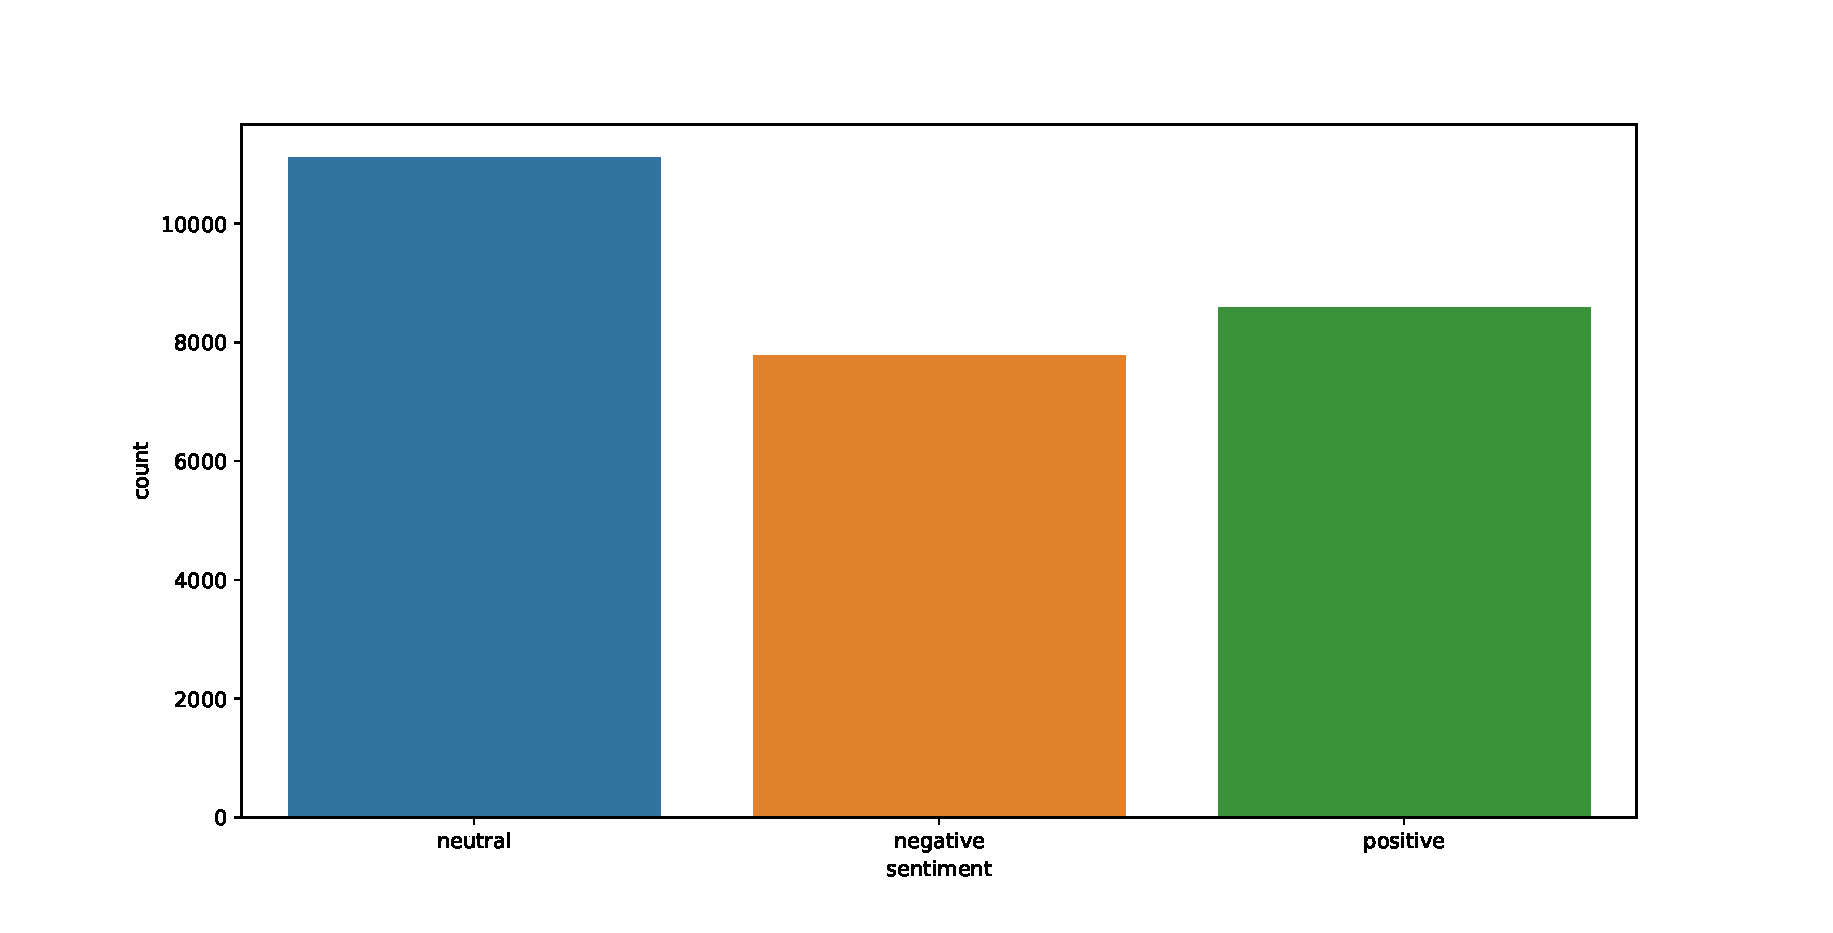
\includegraphics[width=0.9\textwidth]{figures//sentiment.eps}\\
      \vspace{-1.4em}
      \caption{Sentiment}
    \end{minipage}
    \begin{minipage}[t]{0.48\textwidth}
      \centering
      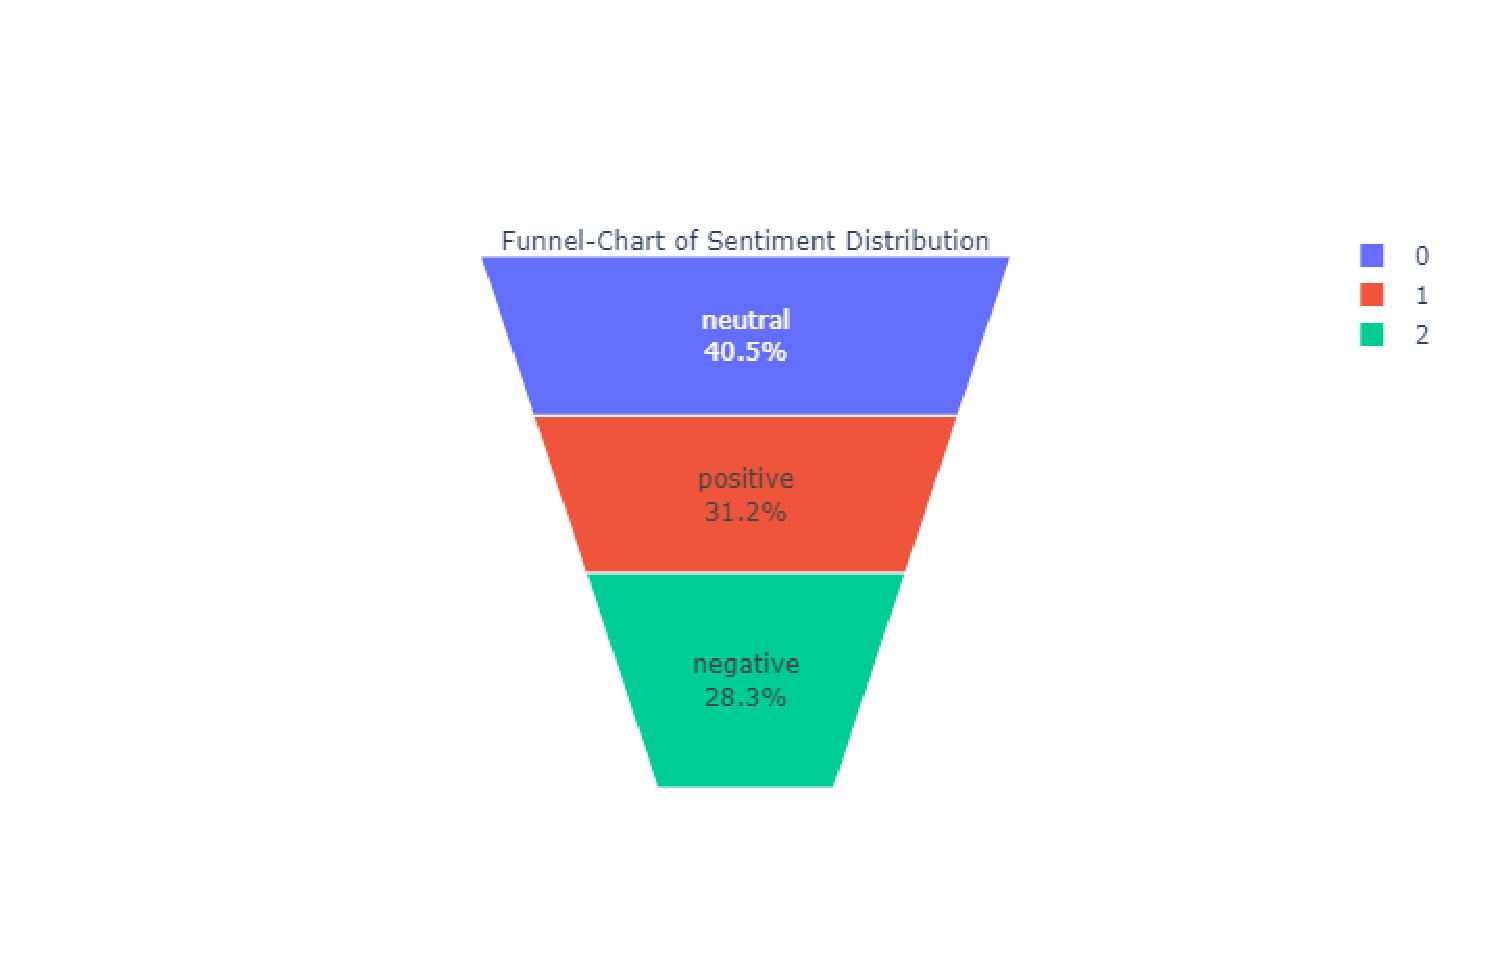
\includegraphics[width=0.9\textwidth]{figures//snetimentdistruct.eps}\\
      \vspace{-1.4em}
      \caption{Sentiment Distribution}
    \end{minipage}
  \end{figure}
\end{slide}
%%
%%==========================================================================================


%%==========================================================================================
%%
\begin{slide}[toc=,bm=]{Selected_text Count}
  \begin{itemize}
    \item After separating selected_text, look at the words used frequently.
  \end{itemize}
  \begin{figure}[htbp]
    \centering
    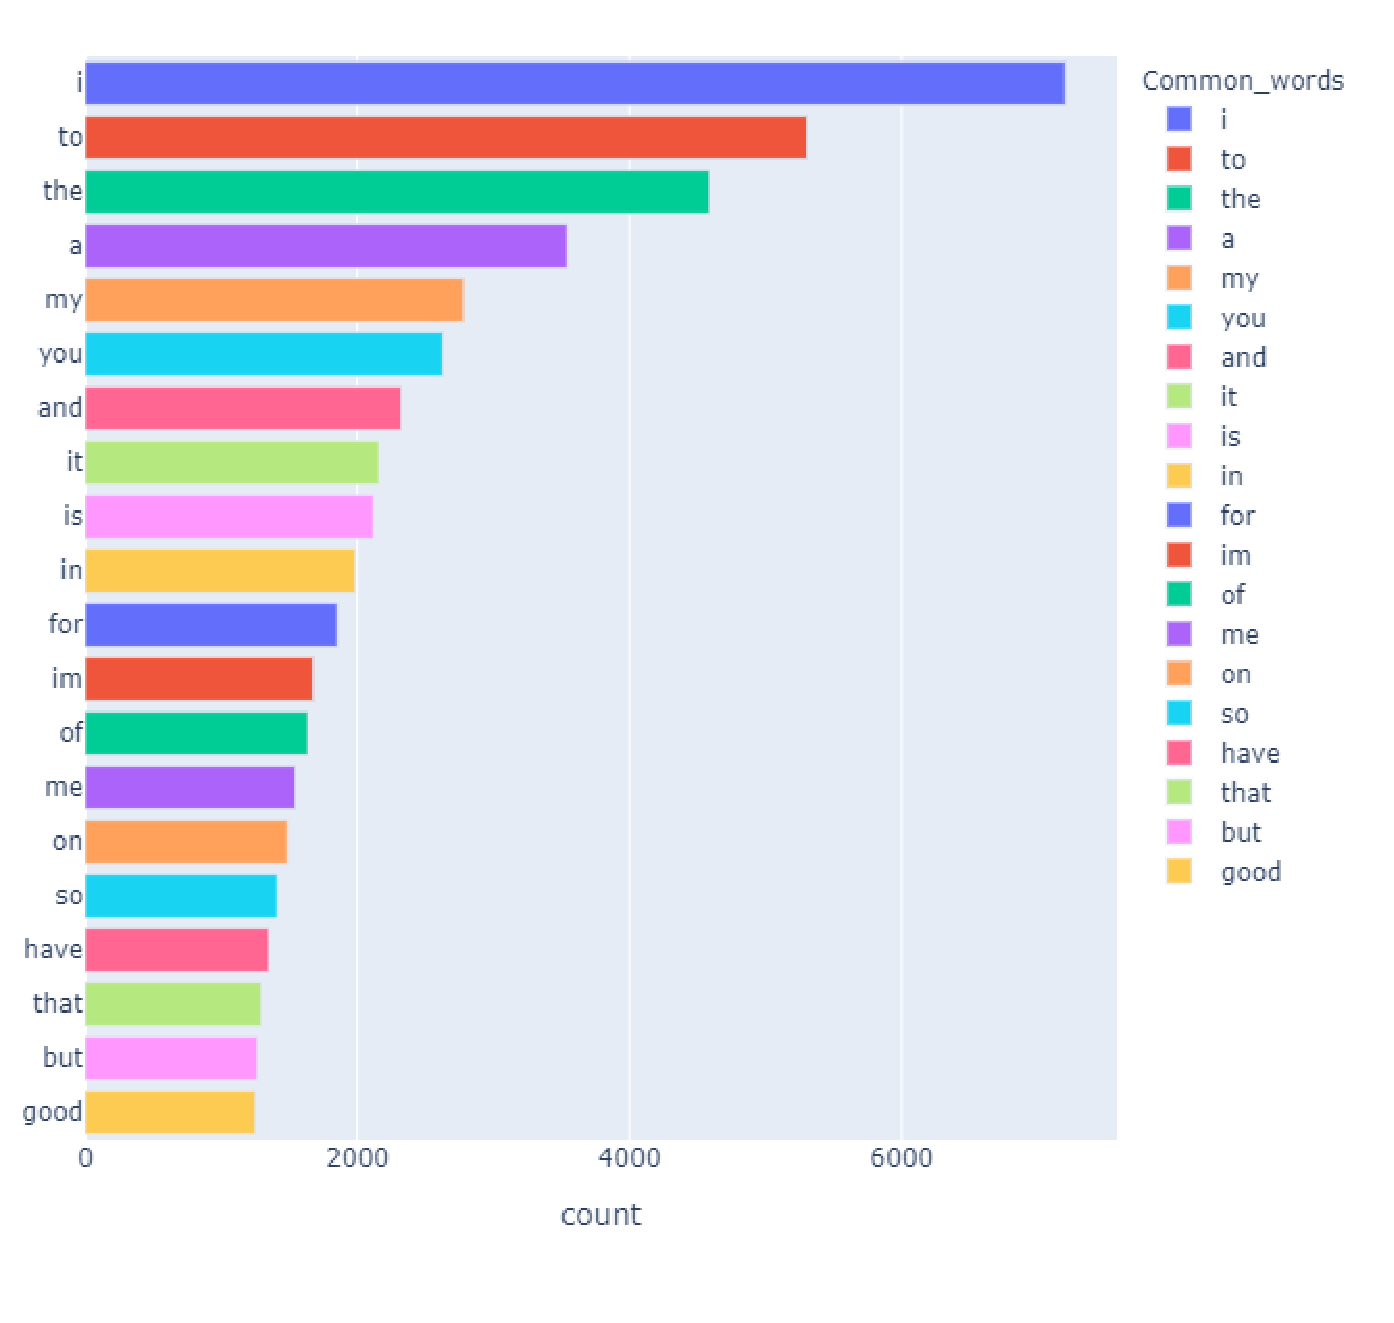
\includegraphics[width=0.5\textwidth]{figures//st_count_test.eps}
    \caption{Select_text Count}
  \end{figure}
\end{slide}
%%
%%==========================================================================================

\begin{slide}[toc=,bm=]{Selected_text Count}
  \begin{itemize}
    \item After processing some irrelevant words, count the number of words.
  \end{itemize}
  \begin{figure}[htbp]
    \centering
    \begin{minipage}[t]{0.48\textwidth}
      \centering
      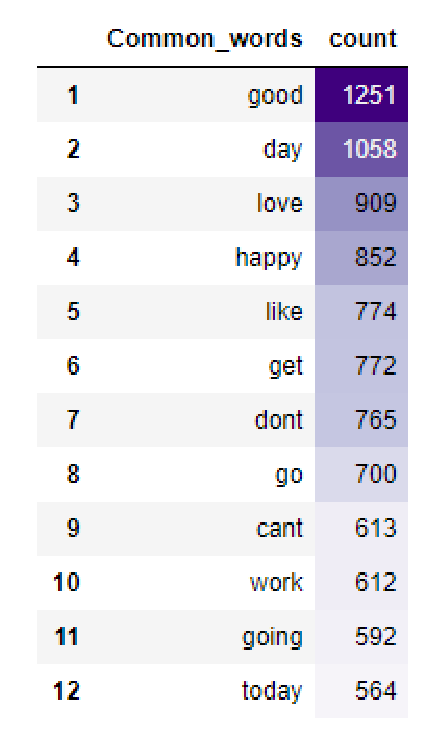
\includegraphics[width=0.5\textwidth]{figures//st_count_new_n.eps}\\
      \vspace{-1.4em}
      \caption{Number Count}
    \end{minipage}
    \begin{minipage}[t]{0.48\textwidth}
      \centering
      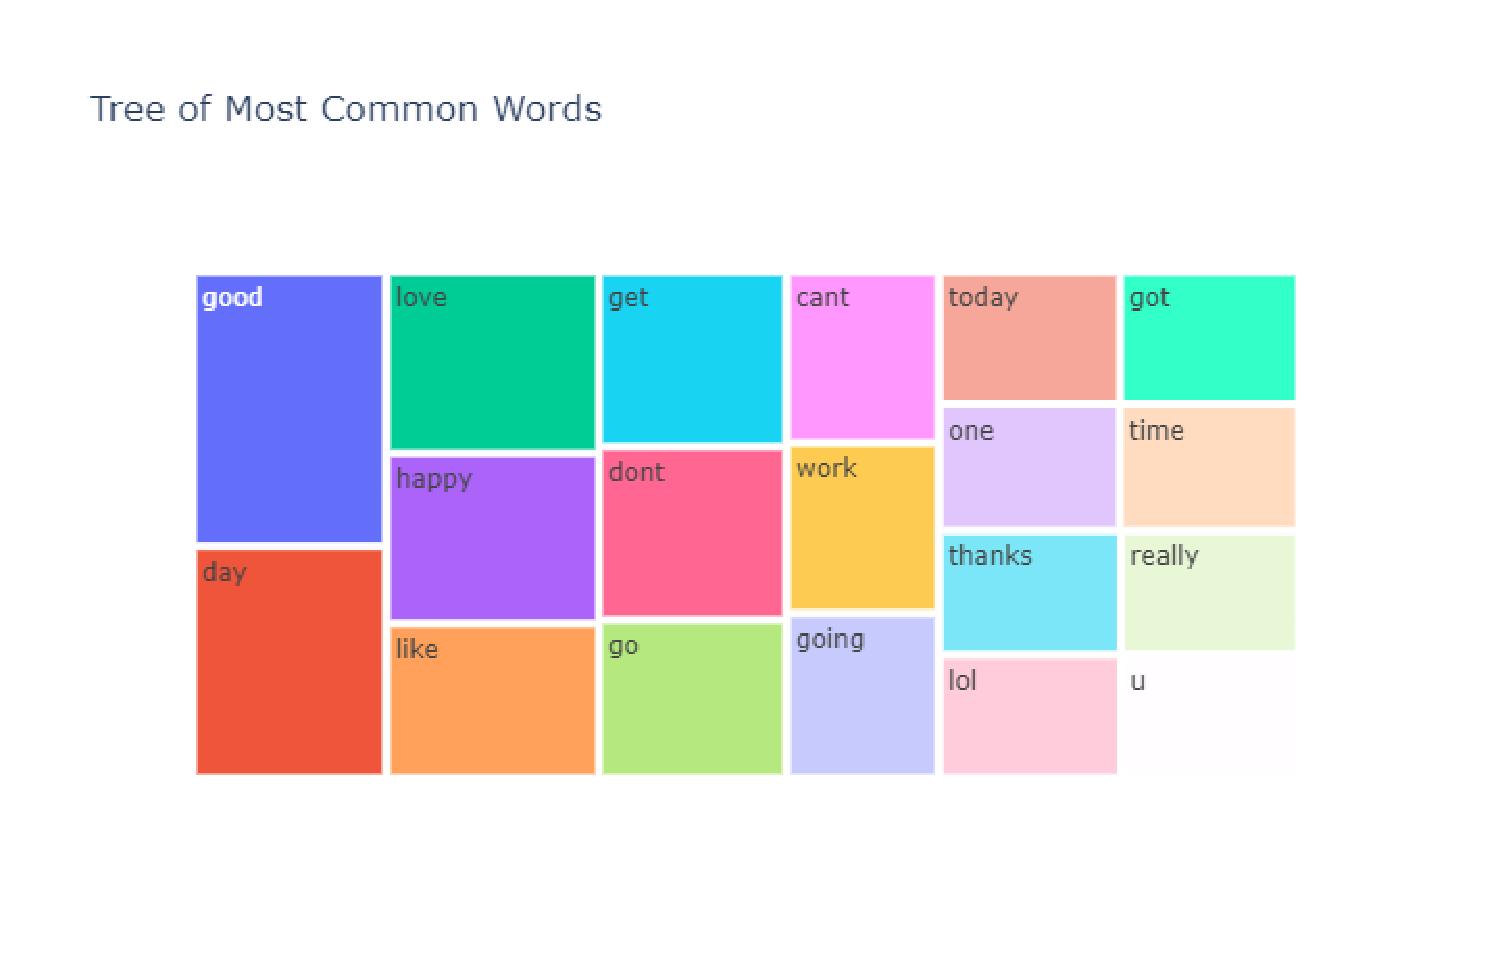
\includegraphics[width=0.9\textwidth]{figures//st_count_new.eps}\\
      \vspace{-1.4em}
      \caption{Tree of Most Common Words}
    \end{minipage}
  \end{figure}
\end{slide}


\begin{slide}{Text Count}
  \begin{itemize}
    \item Count and view the number of text words. Found similar to the selected_text word.
  \end{itemize}
  \begin{figure}[htbp]
    \centering
    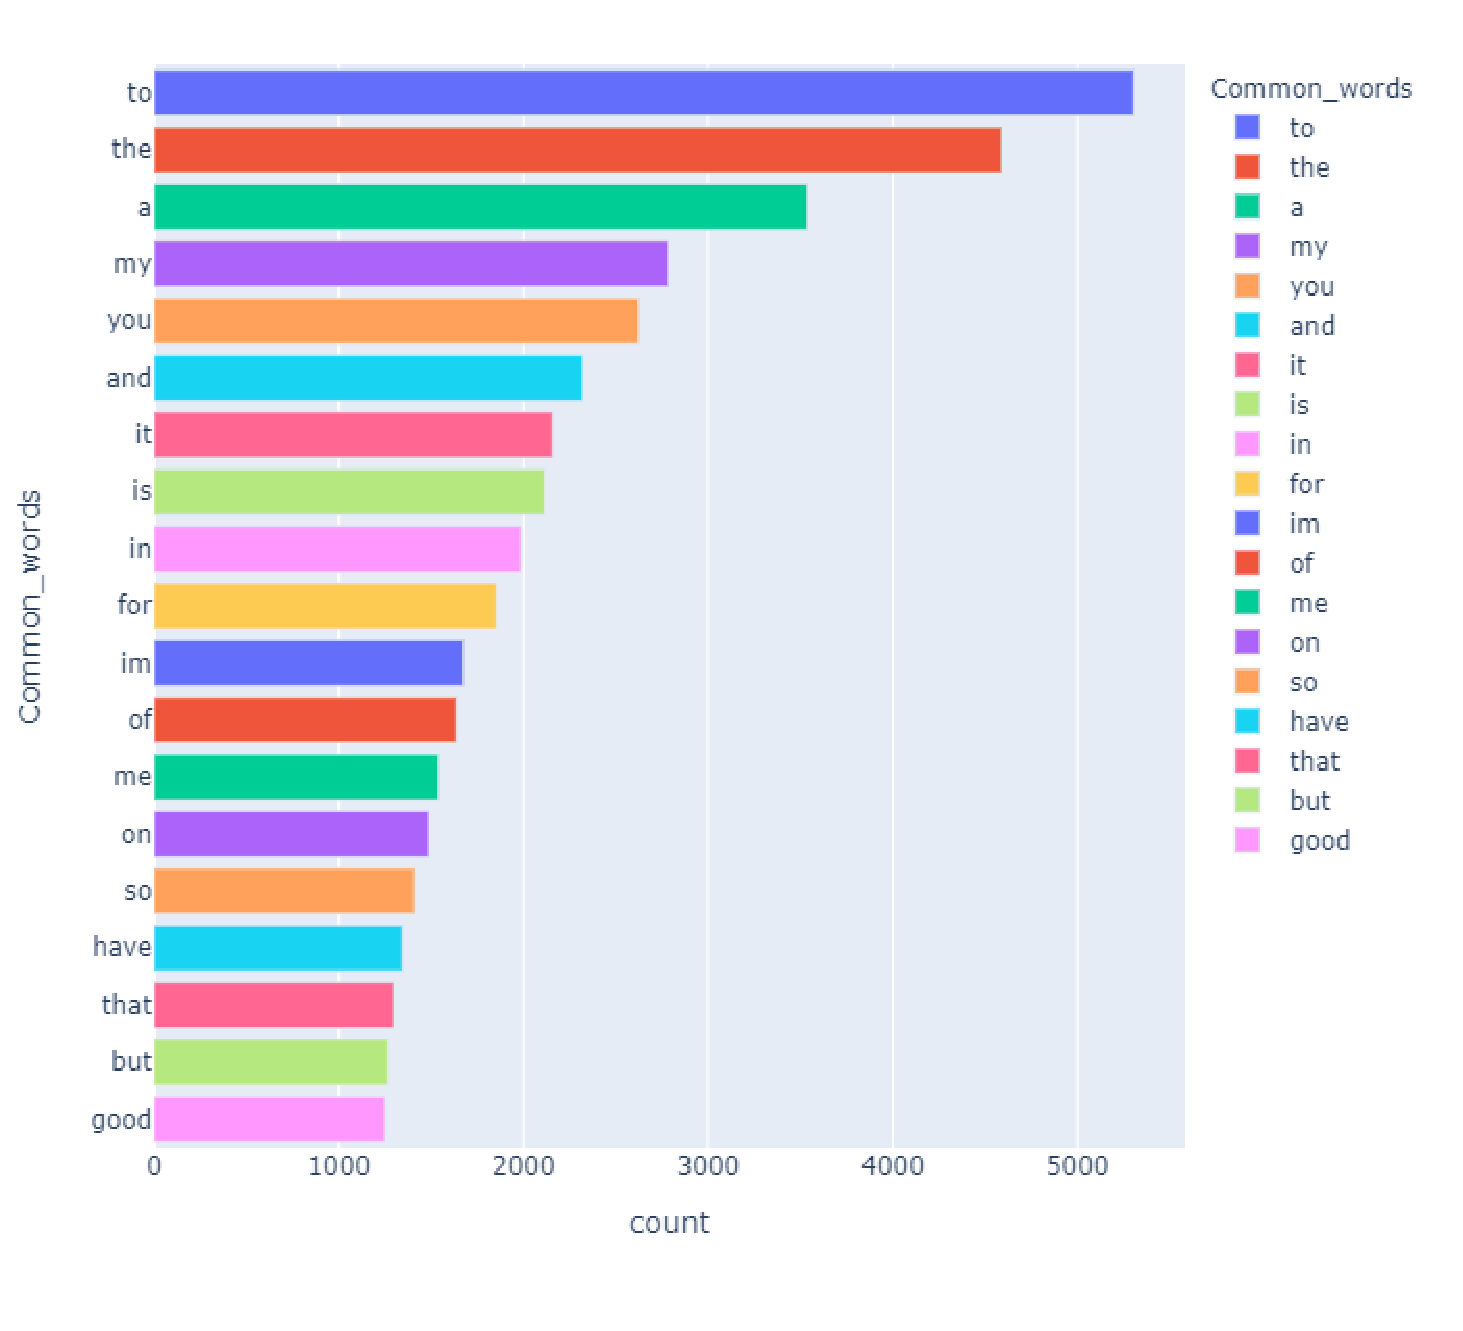
\includegraphics[width=0.5\textwidth]{figures//text_count_test.eps}
    \caption{Text Count}
  \end{figure}
\end{slide}




\begin{slide}{Positive Words}
  \begin{itemize}
    \item Perform word statistics on texts with positive attitudes.
  \end{itemize}
  \begin{figure}[htbp]
    \centering
    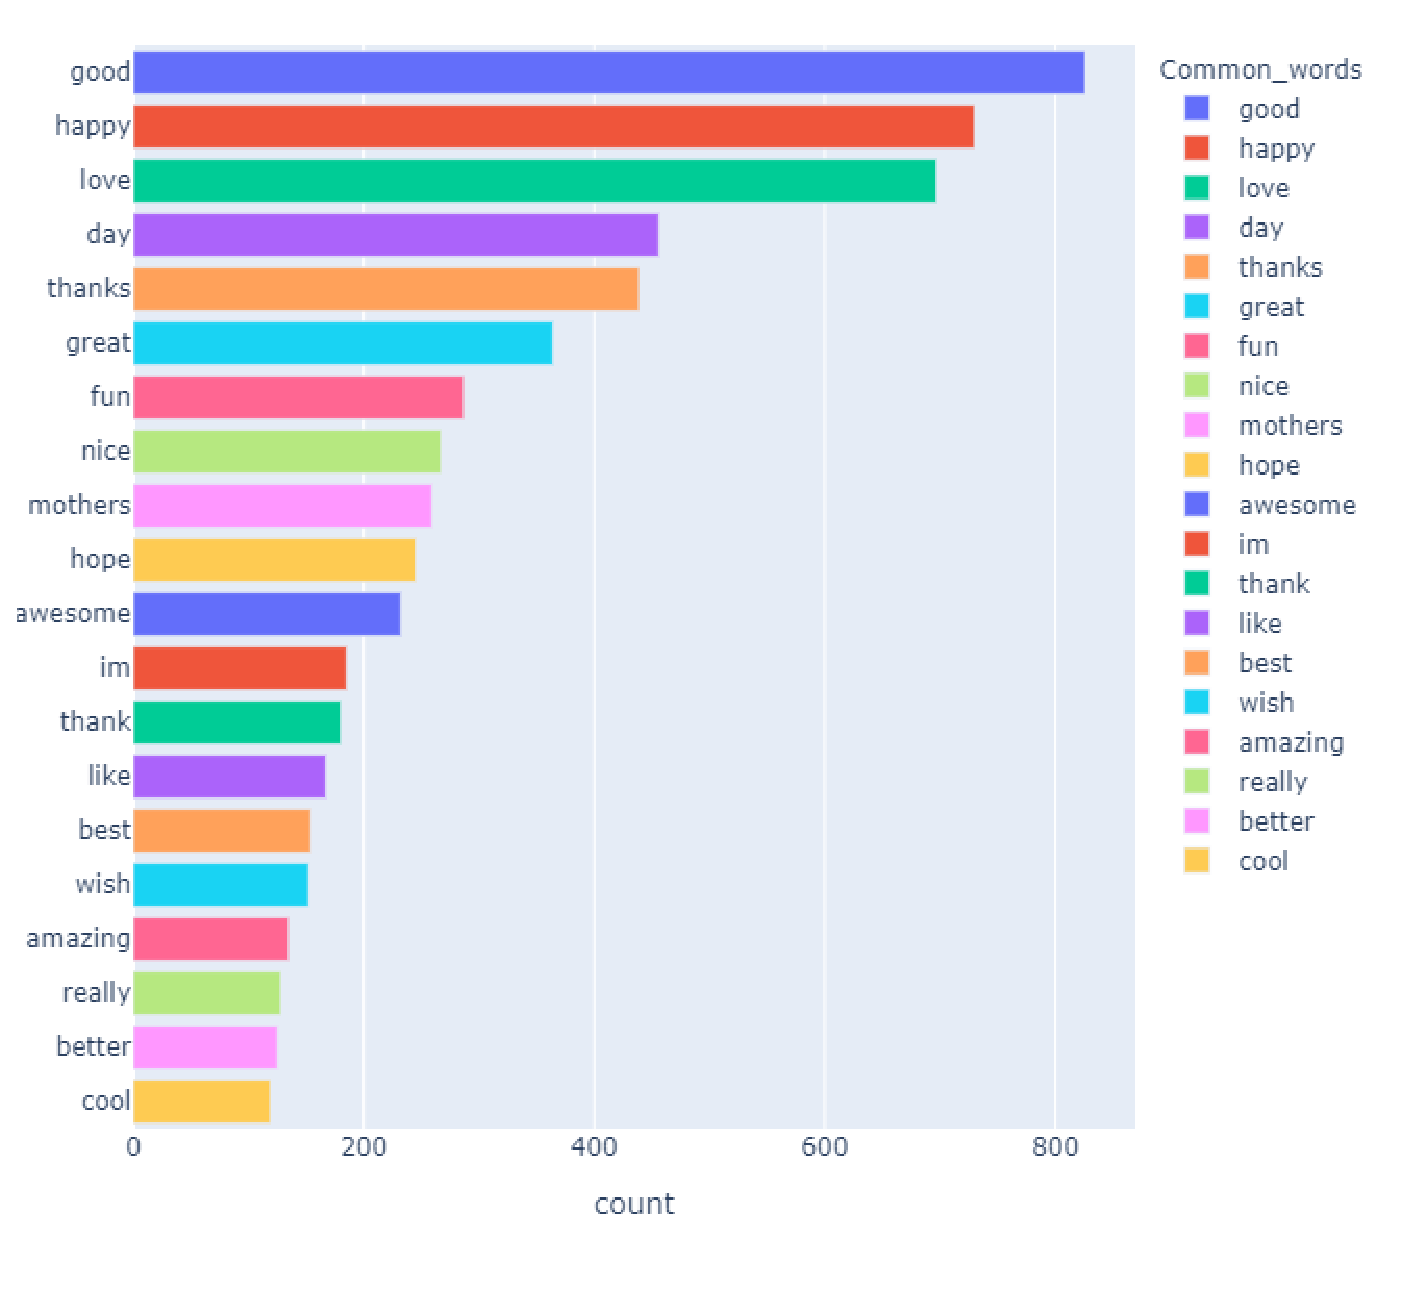
\includegraphics[width=0.5\textwidth]{figures//positive_test.eps}
    \caption{Positive Words}
  \end{figure}
\end{slide}


\begin{slide}{Negative Words}
  \begin{itemize}
    \item Count the words of negative attitude text.
  \end{itemize}
  \begin{figure}[htbp]
    \centering
    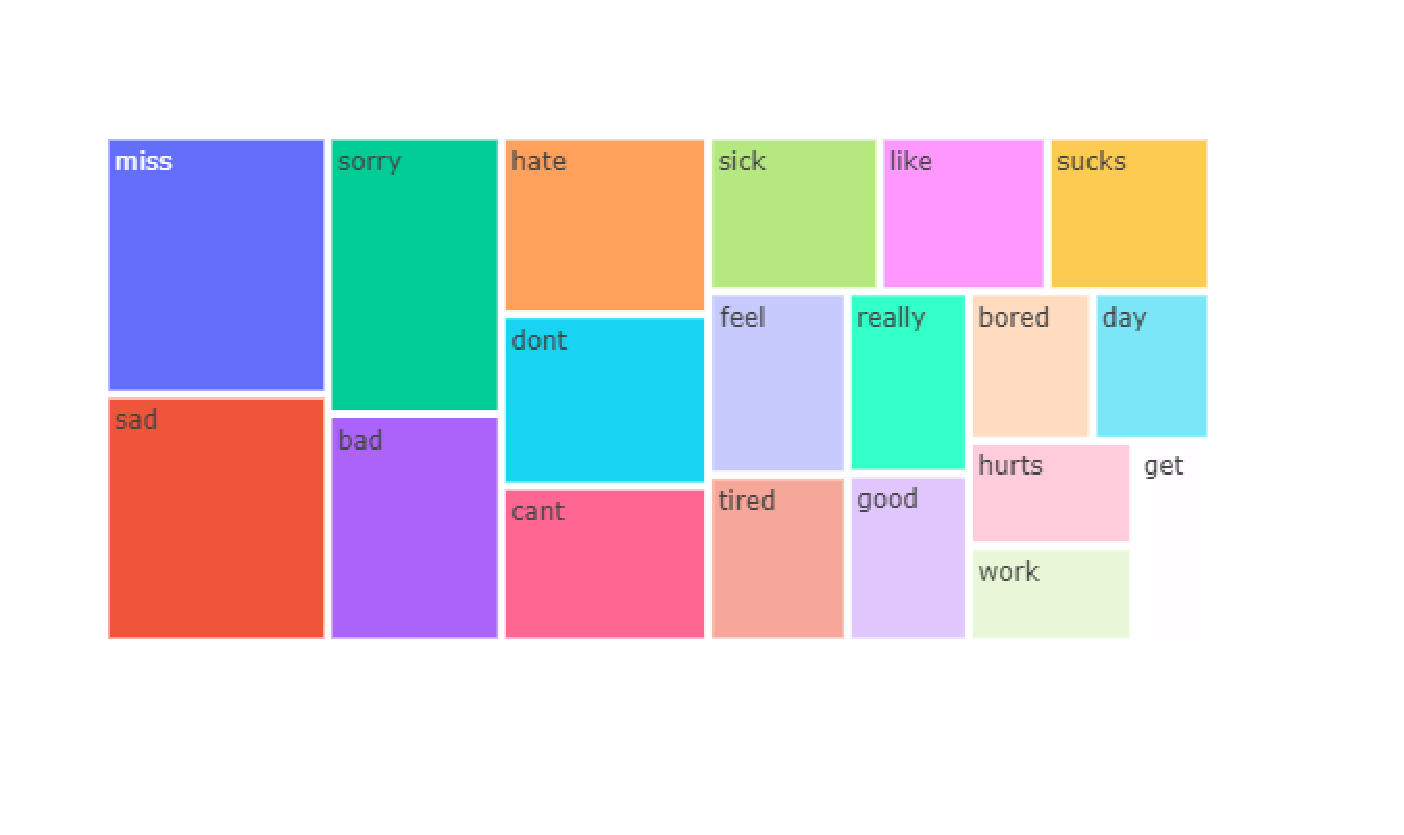
\includegraphics[width=0.8\textwidth]{figures//negative_test.eps}
    \caption{Negative Words}
  \end{figure}
\end{slide}

\begin{slide}[toc=,bm=]{Neutral Words}
  \begin{itemize}
    \item Analyze and display neutral texts.
  \end{itemize}
  \begin{figure}[htbp]
    \centering
    \begin{minipage}[t]{0.48\textwidth}
      \centering
      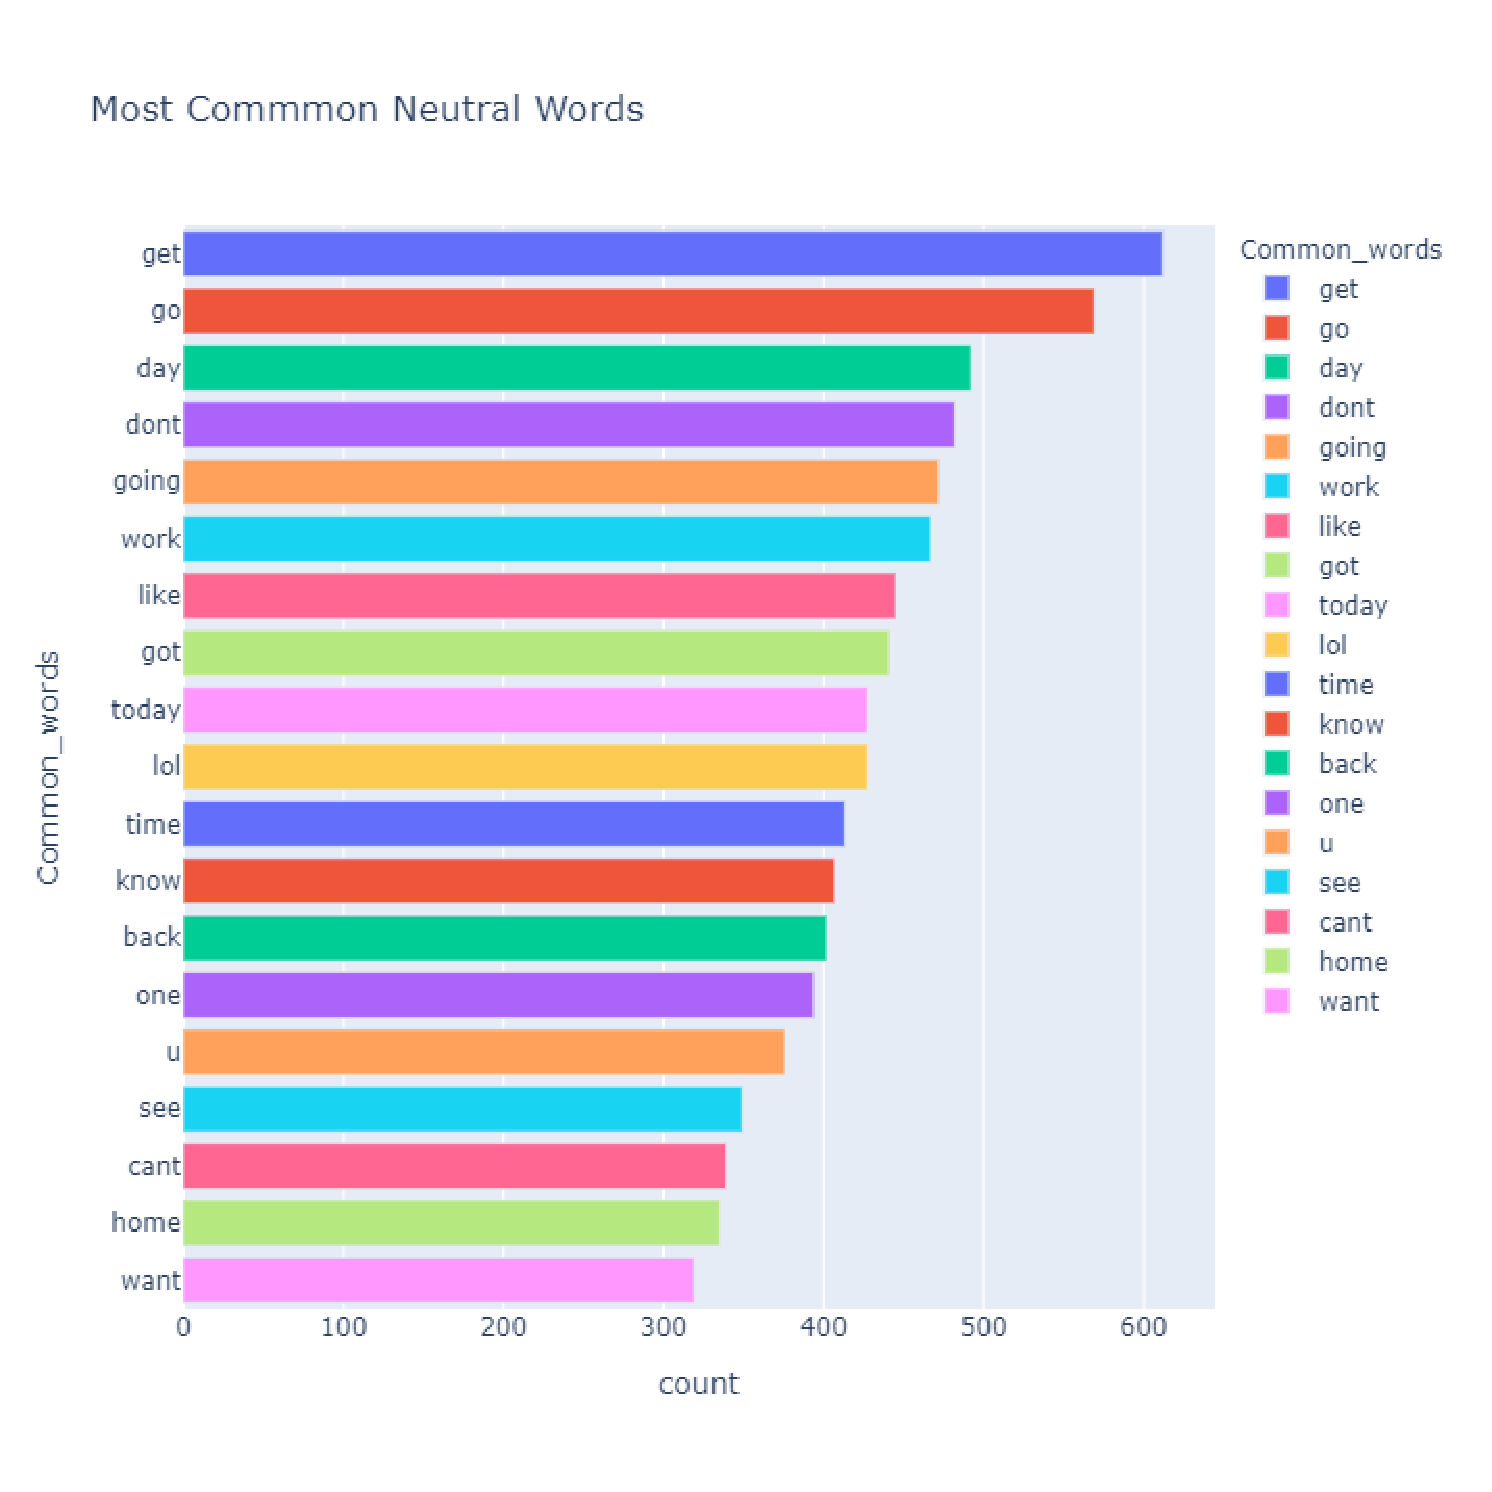
\includegraphics[width=0.9\textwidth]{figures//neutral.eps}
      \vspace{-1.4em}
      \caption{Neutral Words}
    \end{minipage}
    \begin{minipage}[t]{0.48\textwidth}
      \centering
      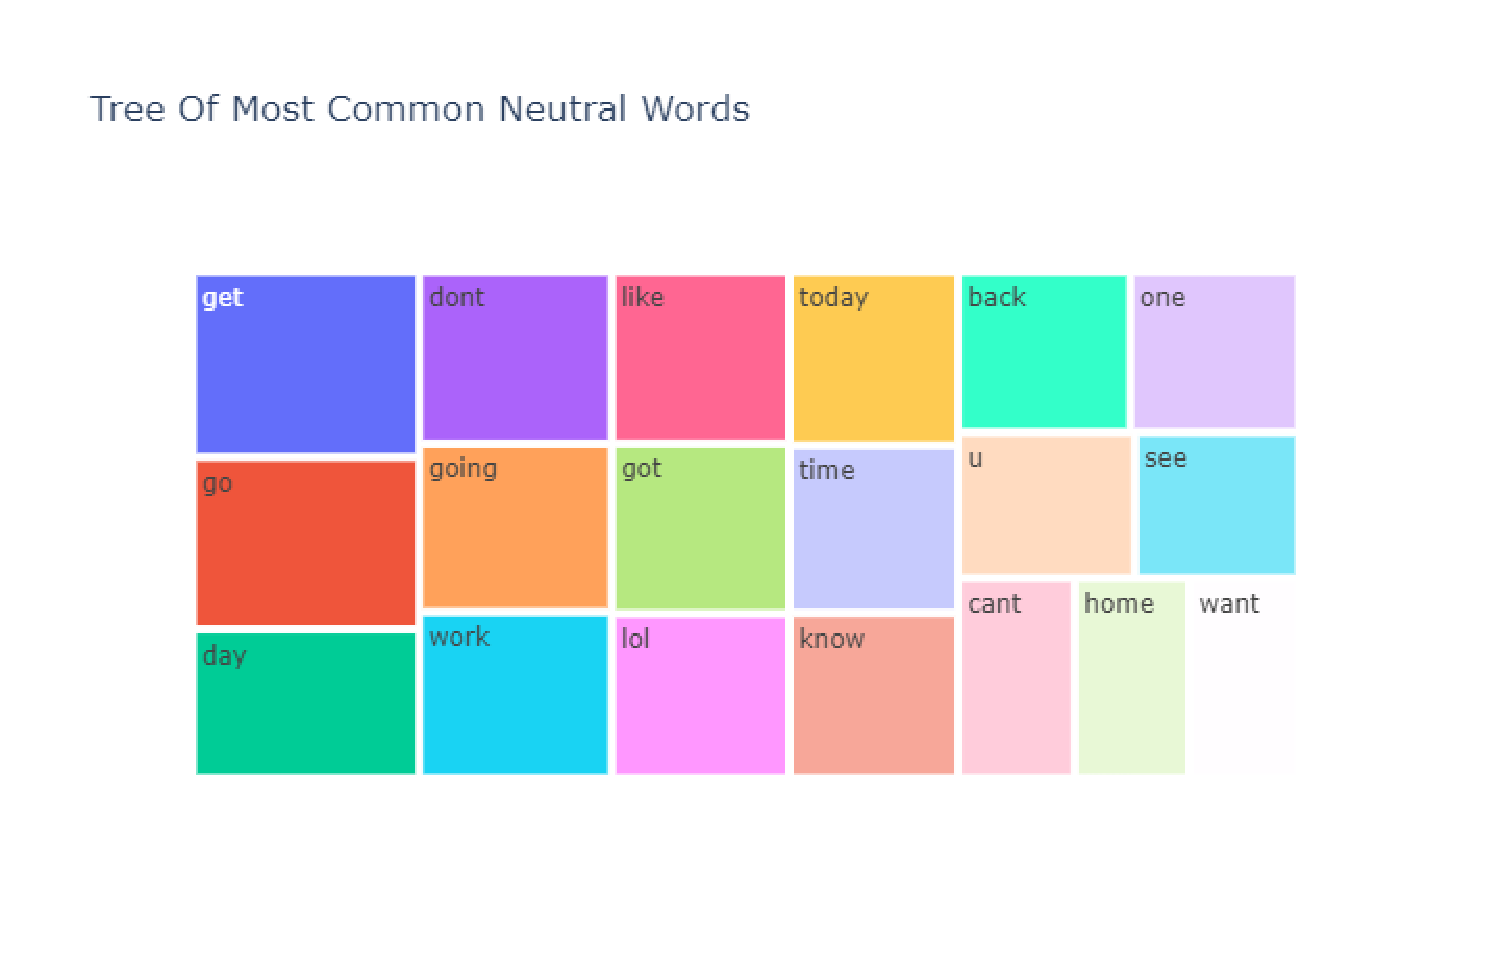
\includegraphics[width=0.9\textwidth]{figures//neutral_tree.eps}
      \vspace{-1.4em}
      \caption{Tree of Most Neutral Words}
    \end{minipage}
  \end{figure}
\end{slide}

%%
%%==========================================================================================


%%==========================================================================================
%%

% \begin{slide}[toc=,bm=]{Propaganda}
%   \begin{itemize}
%     \item Later stage propaganda has a great influence on the existing.
%   \end{itemize}
%   \begin{figure}[htbp]
%     \centering
%     \begin{minipage}[t]{0.48\textwidth}
%       \centering
%       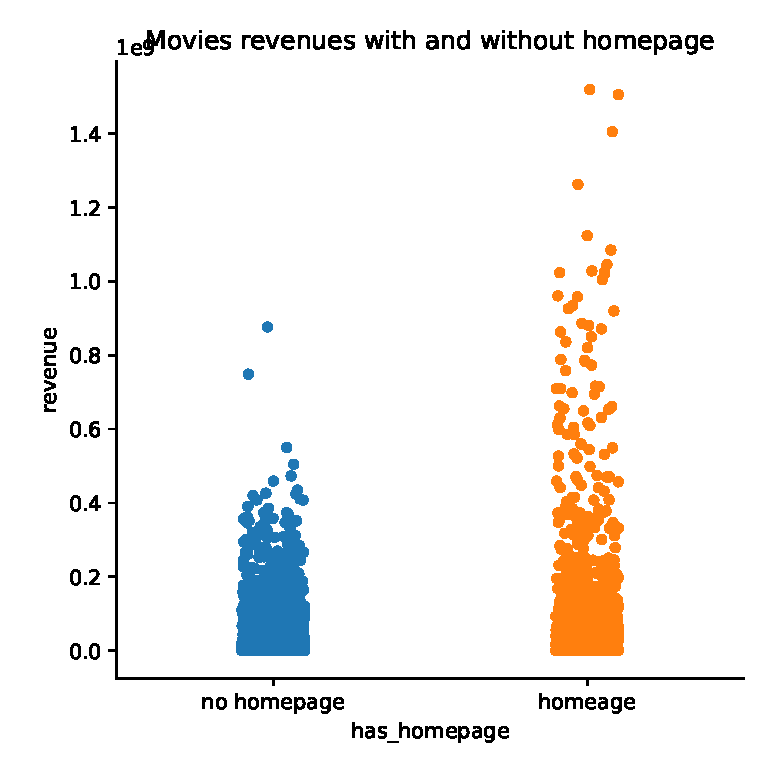
\includegraphics[width=0.4\textwidth]{figures/has_homepage.eps}
%       \vspace{-1.4em}
%       \caption{Homepage}
%     \end{minipage}
%     \begin{minipage}[t]{0.48\textwidth}
%       \centering
%       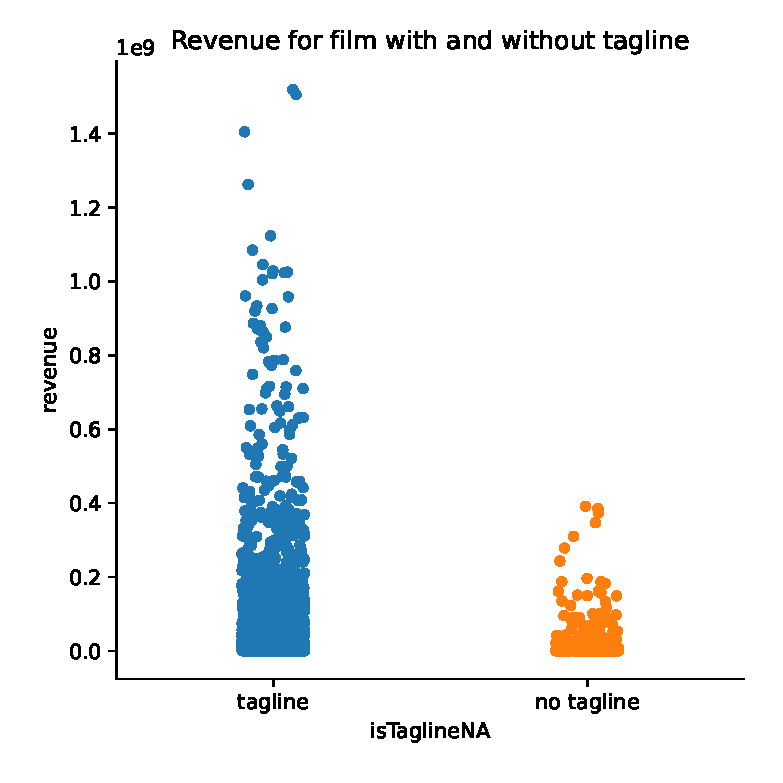
\includegraphics[width=0.4\textwidth]{figures/isTanglineNA.eps}
%       \vspace{-1.4em}
%       \caption{Tagline}
%     \end{minipage}
%     \begin{minipage}[t]{0.48\textwidth}
%       \centering
%       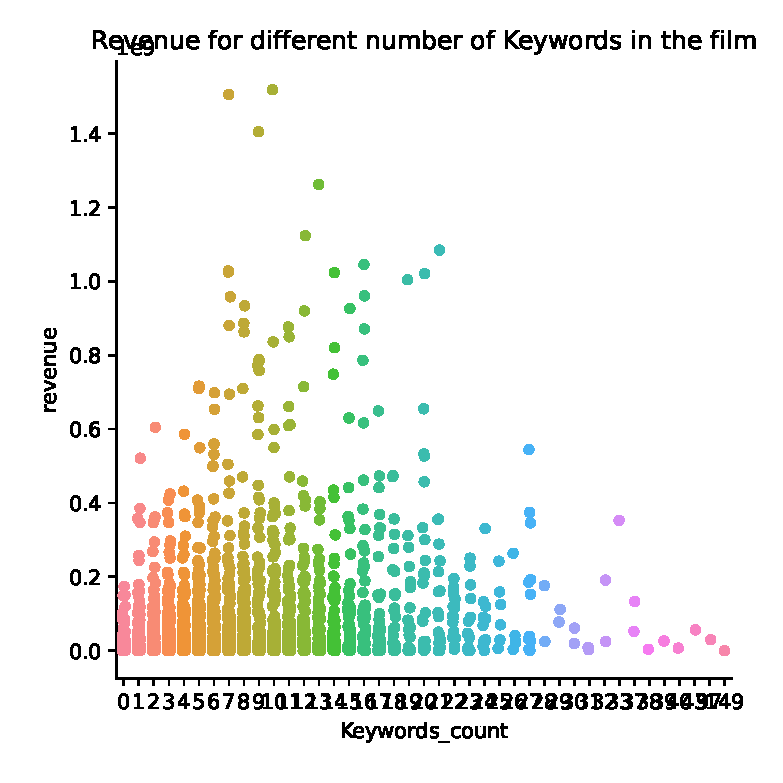
\includegraphics[width=0.5\textwidth]{figures/keywords.eps}
%       \vspace{-1.4em}
%       \caption{keywords}
%     \end{minipage}
%     \begin{minipage}[t]{0.48\textwidth}
%       \centering
%       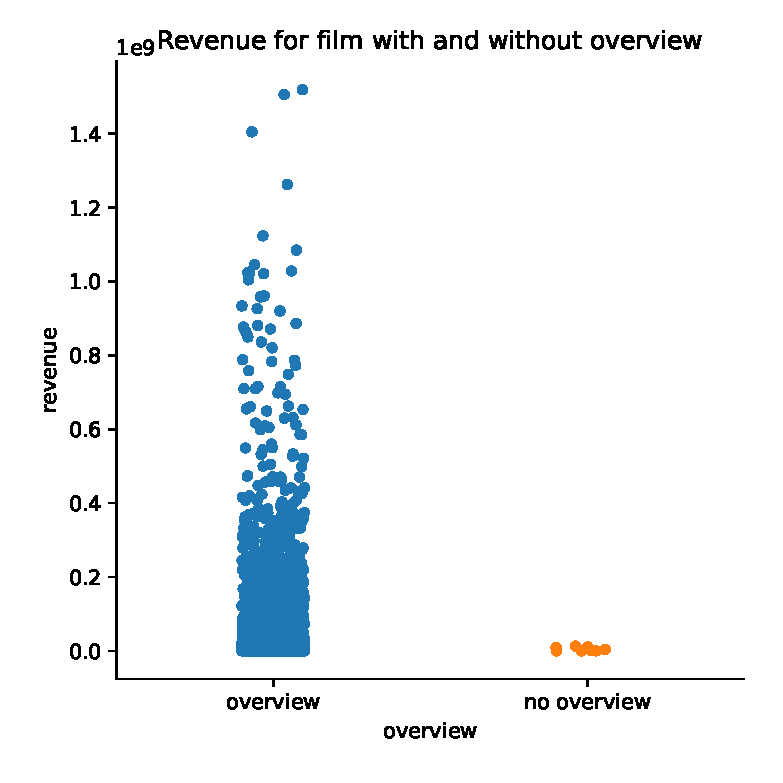
\includegraphics[width=0.5\textwidth]{figures/overview.eps}
%       \vspace{-1.4em}
%       \caption{Overview}
%     \end{minipage}
%   \end{figure}
% \end{slide}


%%==========================================================================================
%%
% \begin{slide}[toc=,bm=]{Realte Date}
% %  \begin{itemize}
% %    \item The income of the film is directly proportional to the budget.
% %  \end{itemize}
%   \begin{figure}[htbp]
%     \centering
%     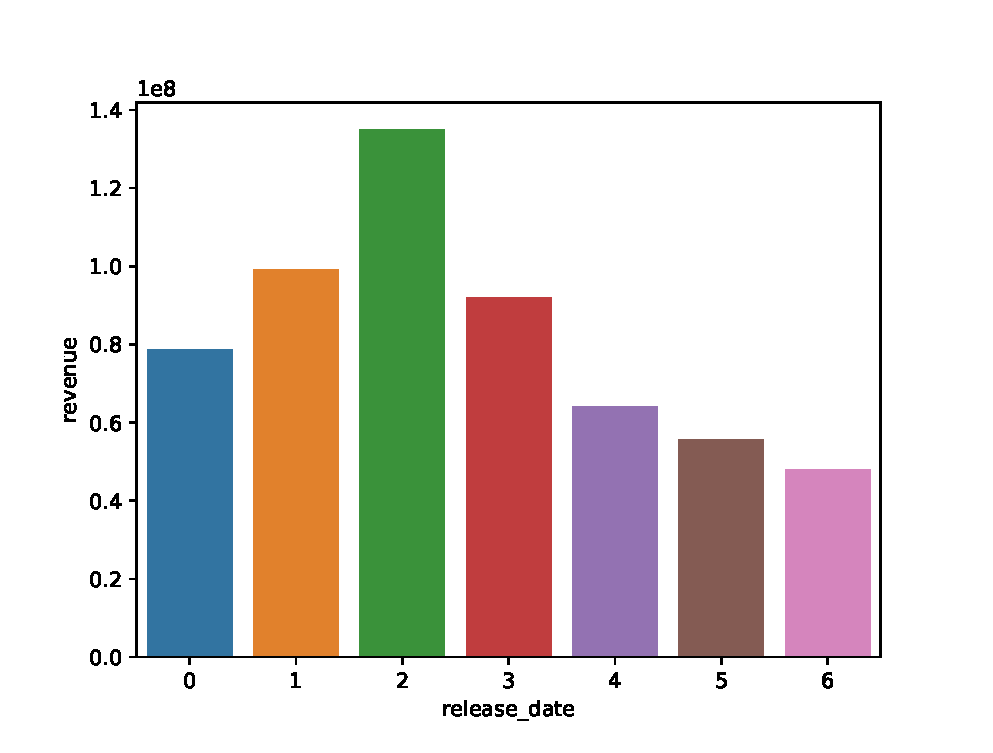
\includegraphics[width=0.7\textwidth]{figures//release_date.eps}
%     \caption{Realte Date}
%   \end{figure}
% \end{slide}
% %%


% \section{Data Processing}


% \begin{slide}[toc=,bm=]{Data Processing}
%   \begin{itemize}
%     \item Processing data independent of results.
%       \begin{itemize}
%         \item For example:imdb_id,orginal_title,poster_path,status
%       \end{itemize}
%     \item  Normalization of training data and test data.
%       \begin{itemize}
%         \item For example:has_homepage,collection,overview,isTaglineNA,Keywords_count etc
%       \end{itemize}
%   \end{itemize}
%   \begin{table}[htbp]
%     \caption{Delete Data}
%     \begin{tabular}{p{100pt} | p{200pt}}\toprule
%      Name & Description  \\
%          \midrule
%          imdb_id
%          & ID of movie in TMDB \\
%          orginal_title
%          & The original name of the movie\\
%          poster_path
%          & Movie poster link \\
%          status
%          &The state of the film \\
%         \bottomrule
%     \end{tabular}
%    \end{table}
% \end{slide}
% %%


% \section{Modeling and Forecasting}


% %%
% \begin{slide}[toc=,bm=]{Model}

% \begin{itemize}
%   \item Linear Regression
%      \begin{itemize}
%        \item 2.4236034243650315
%      \end{itemize}  
%   \item Random Forest Regression
%      \begin{itemize}
%        \item 2.21274632296787
%      \end{itemize}
% \end{itemize}

% \end{slide}
% %%
% %%==========================================================================================



% %%
% \begin{slide}{Forecast}

% \begin{itemize}
% \item Random forest regression algorithm makes prediction.
% \end{itemize}

% \begin{table}
% \centering
% \caption{Forecast Results}

% \begin{tabular}{p{65pt} | p{110pt}}
% \toprule
%   id & revenue\\
% \hline
%   3001 & 193077.0567 \\
%   3002 & 528484.58  \\
%   3003 & 4562948.933  \\
%   3004 &  14433891.04 \\
%   3005 &  494782.0824  \\
%   3006 &  3010483.492  \\
% \bottomrule

% \end{tabular}
% \end{table}

% \end{slide}


% %%
% %%==========================================================================================


% \section{Conclusion}

% %%==========================================================================================
% %%
% \begin{slide}[toc=,bm=]{Conclusion}
% \begin{itemize}
% \item The investment in the early stage and publicity in the later stage have an impact on the box office.
% \smallskip

% \item
% \smallskip
% In the early stage, the number of actors and crew should be moderate, not the more the better.

% \item
% \smallskip
% The prediction accuracy can be further improved, such as using XGBoost
% \end{itemize}

% \end{slide}
%%
%%==========================================================================================


%%==========================================================================================
% TODO: Contact Page
%\begin{wideslide}[toc=,bm=]{Contact Information}
%\centering
%\vspace{\stretch{1}}
%\twocolumn[
%lcolwidth=0.35\linewidth,
%rcolwidth=0.65\linewidth
%]
%{
% \centerline{
\includegraphics[scale=.2]{tulip-logo.eps}}
%}
%{
%\vspace{\stretch{1}}
%Associate Professor Gang Li\\
%School of Information Technology\\
%Deakin University, Australia
%\begin{description}
% \item[\textcolor{orange}{\faEnvelope}] \href{mailto:gangli@tulip.org.au}
% {\textsc{\footnotesize{gangli@tulip.org.au}}}
%
% \item[\textcolor{orange}{\faHome}] \href{http://www.tulip.org.au}
% {\textsc{\footnotesize{Team for Universal Learning and Intelligent Processing}}}
%\end{description}
%}
%\vspace{\stretch{1}}
%\end{wideslide}
%
\end{document}

\endinput
